\subsection{Matriz Morfológica}


 Es una herramienta que  permite comparar diferentes principios de solución para cada una de las diferentes partes de una máquina. A través de las distintas opciones que se proponen se pueden plantear diferentes alternativas en el proceso de diseño.
 Se utilizará la matriz morfológica (Tabla \ref{tab:morfologica}).

\begin{table}[h!]
    \begin{center}
    \caption{Matriz morfológica para el diseño del sistema de compostaje}
    \resizebox{16cm}{!}{
            \begin{tabular}{ |c|c|c|c|c| } 
            %\hline
                %\multicolumn{5}{|c|}{Propuestas de diseño} \\
            \hline
                 Función & Opción A & Opción B & Opción C & Opción D \\ \hline
                 Trituración & 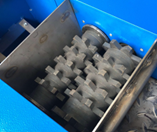
\includegraphics[scale=0.2]{images/Capitulo 3/3.1.2.1 Matriz morfologica/1A.png} & 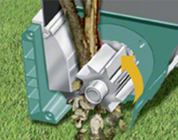
\includegraphics[scale=0.2]{images/Capitulo 3/3.1.2.1 Matriz morfologica/1B.png} & 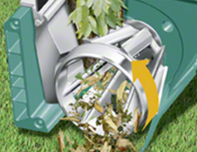
\includegraphics[scale=0.2]{images/Capitulo 3/3.1.2.1 Matriz morfologica/1C.png} & 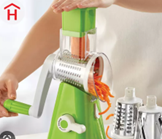
\includegraphics[scale=0.2]{images/Capitulo 3/3.1.2.1 Matriz morfologica/1D.png} \\ \hline
                 Almacenamiento & 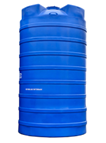
\includegraphics[scale=0.2]{images/Capitulo 3/3.1.2.1 Matriz morfologica/2A.png} & 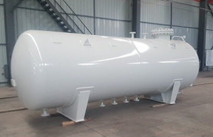
\includegraphics[scale=0.2]{images/Capitulo 3/3.1.2.1 Matriz morfologica/2B.png} &  &  \\ \hline
                 Palas de agitación & 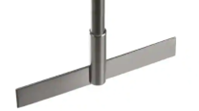
\includegraphics[scale=0.3]{images/Capitulo 3/3.1.2.1 Matriz morfologica/3A.png} & 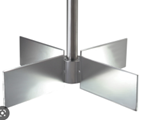
\includegraphics[scale=0.3]{images/Capitulo 3/3.1.2.1 Matriz morfologica/3B.png} & 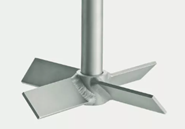
\includegraphics[scale=0.3]{images/Capitulo 3/3.1.2.1 Matriz morfologica/3C.png} & 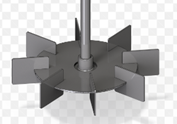
\includegraphics[scale=0.3]{images/Capitulo 3/3.1.2.1 Matriz morfologica/3D.png} \\ \hline
                 Transmisión de movimiento & 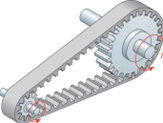
\includegraphics[scale=0.3]{images/Capitulo 3/3.1.2.1 Matriz morfologica/4A.png} & 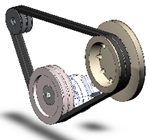
\includegraphics[scale=0.3]{images/Capitulo 3/3.1.2.1 Matriz morfologica/4B.png} & 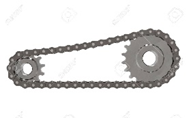
\includegraphics[scale=0.3]{images/Capitulo 3/3.1.2.1 Matriz morfologica/4C.png} & 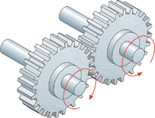
\includegraphics[scale=0.3]{images/Capitulo 3/3.1.2.1 Matriz morfologica/4D.png} \\ \hline
                 Medir Temperatura & 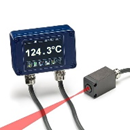
\includegraphics[scale=0.3]{images/Capitulo 3/3.1.2.1 Matriz morfologica/5A.png} & 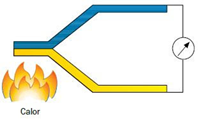
\includegraphics[scale=0.3]{images/Capitulo 3/3.1.2.1 Matriz morfologica/5B.png} & 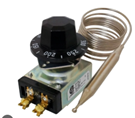
\includegraphics[scale=0.3]{images/Capitulo 3/3.1.2.1 Matriz morfologica/5C.png} & 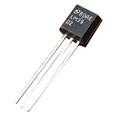
\includegraphics[scale=0.3]{images/Capitulo 3/3.1.2.1 Matriz morfologica/5D.png} \\ \hline
                 Medir humedad & 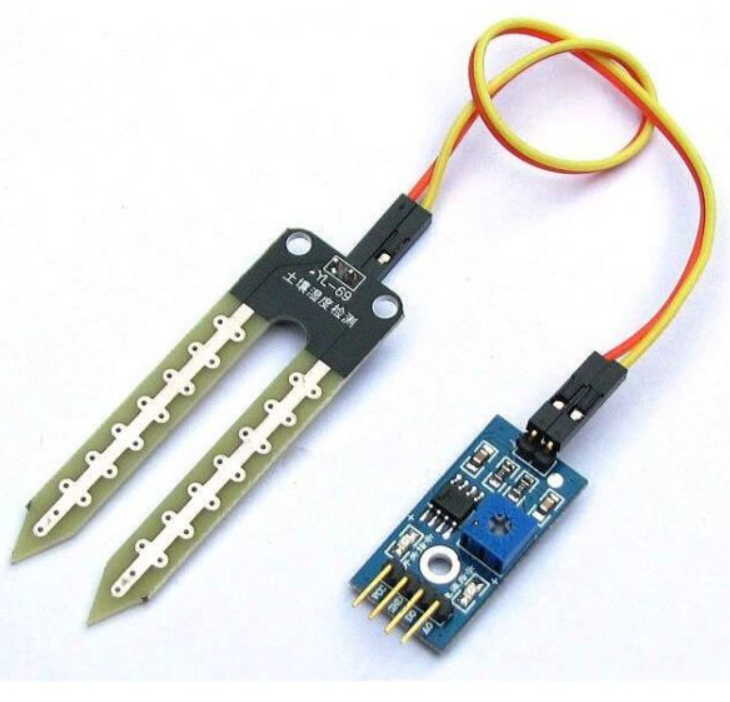
\includegraphics[scale=0.06]{images/Capitulo 3/3.1.2.1 Matriz morfologica/6A.png} & 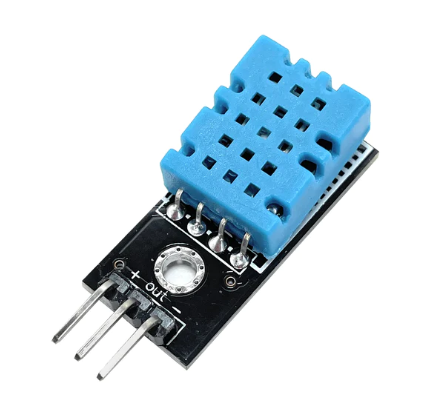
\includegraphics[scale=0.11]{images/Capitulo 3/3.1.2.1 Matriz morfologica/6B.png} &  &  \\ \hline
                 Elevar la temperatura & 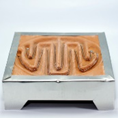
\includegraphics[scale=0.3]{images/Capitulo 3/3.1.2.1 Matriz morfologica/8A.png} & 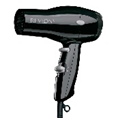
\includegraphics[scale=0.3]{images/Capitulo 3/3.1.2.1 Matriz morfologica/8B.png} & 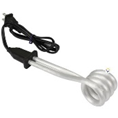
\includegraphics[scale=0.3]{images/Capitulo 3/3.1.2.1 Matriz morfologica/8C.png} &  \\ \hline
                Elevar la humedad & 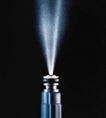
\includegraphics[scale=0.3]{images/Capitulo 3/3.1.2.1 Matriz morfologica/9A.png} & 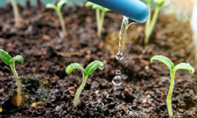
\includegraphics[scale=0.3]{images/Capitulo 3/3.1.2.1 Matriz morfologica/9B.png} & 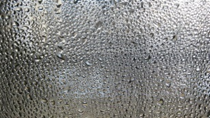
\includegraphics[scale=0.3]{images/Capitulo 3/3.1.2.1 Matriz morfologica/9C.png} &  \\ \hline
                 Oxigenar el sistema & 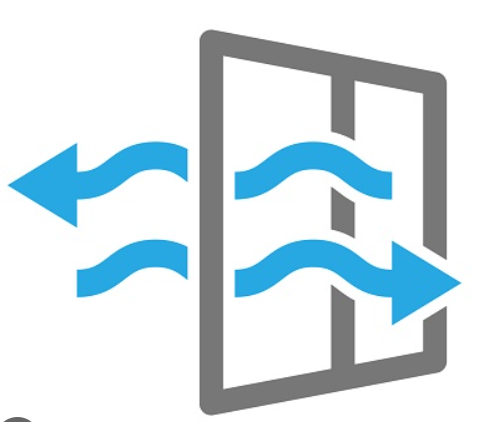
\includegraphics[scale=0.10]{images/Capitulo 3/3.1.2.1 Matriz morfologica/10A.png} & 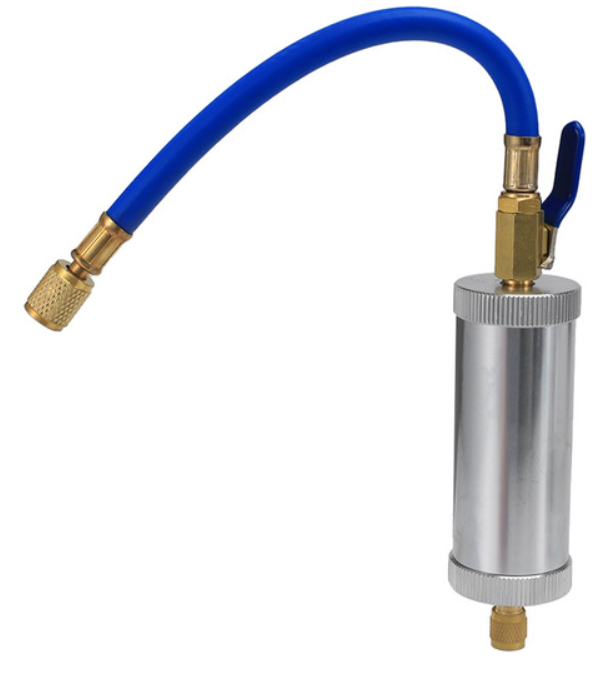
\includegraphics[scale=0.07]{images/Capitulo 3/3.1.2.1 Matriz morfologica/10B.png} &  &  \\ \hline
        \end{tabular}
        }
    \end{center}
    \label{tab:morfologica}%
\end{table}

\begin{table}[h!]
    \begin{center}
    \resizebox{16cm}{!}{
            \begin{tabular}{ |c|c|c|c|c| } 
            \hline
                 Unidad de procesamiento & 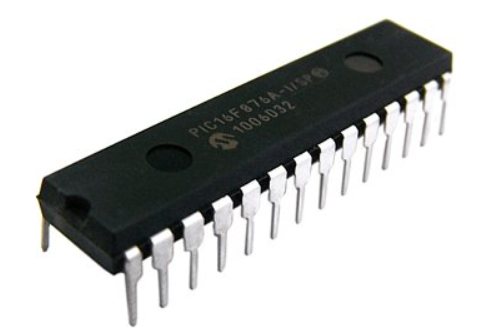
\includegraphics[scale=0.10]{images/Capitulo 3/3.1.2.1 Matriz morfologica/11A.png} & 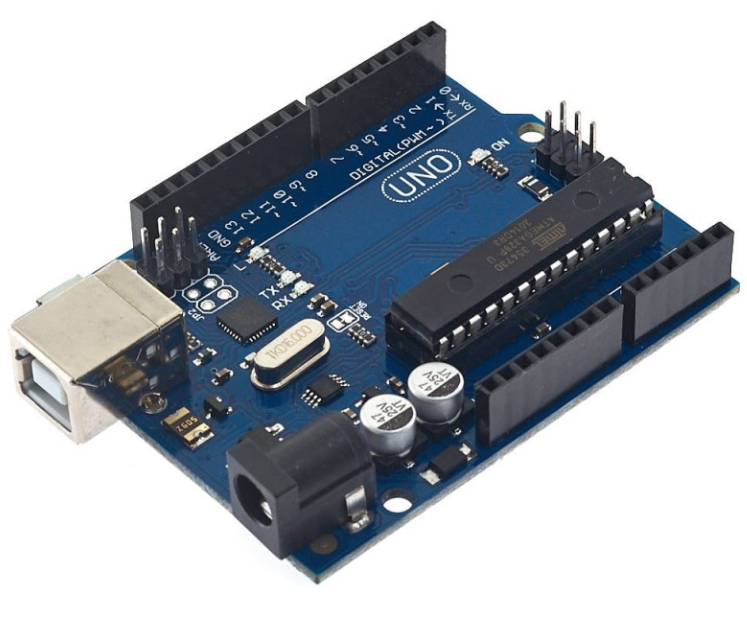
\includegraphics[scale=0.08]{images/Capitulo 3/3.1.2.1 Matriz morfologica/11B.png} & 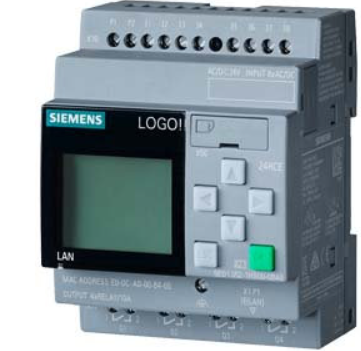
\includegraphics[scale=0.15]{images/Capitulo 3/3.1.2.1 Matriz morfologica/11C.png} &  \\ \hline
                 Interfaz HM & 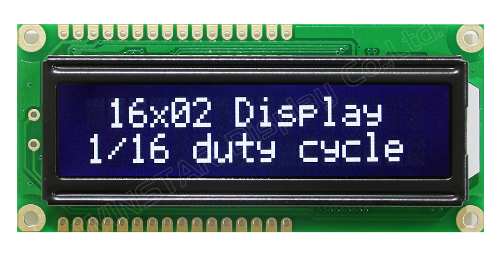
\includegraphics[scale=0.15]{images/Capitulo 3/3.1.2.1 Matriz morfologica/12A.png} & 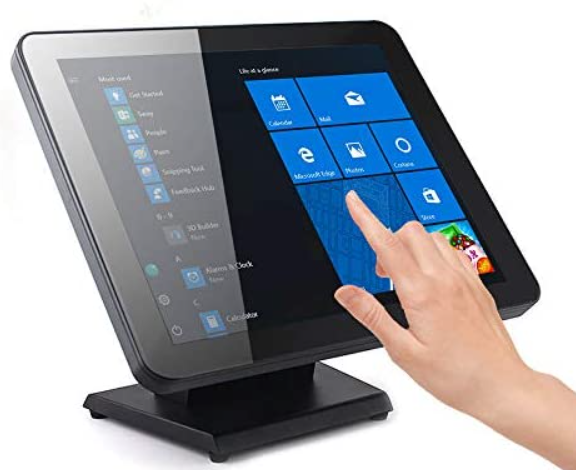
\includegraphics[scale=0.10]{images/Capitulo 3/3.1.2.1 Matriz morfologica/12B.png} & 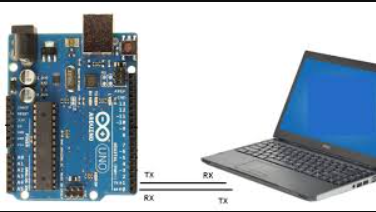
\includegraphics[scale=0.20]{images/Capitulo 3/3.1.2.1 Matriz morfologica/12C.png} & 
\includegraphics[scale=0.20]{images/Capitulo 3/3.1.2.1 Matriz morfologica/12D.png} \\
             \hline
        \end{tabular}
        }
    \end{center}
    \label{tab:morfologica}%
\end{table}
\newpage